\chapter{Introduction}
\vspace{-1cm}
\epigraphfontsize{\small\itshape}
\epigraph{“...if we were to name the most powerful assumption of all, which leads one on
and on in an attempt to understand life, it is that all things are made of atoms, and
that everything that living things do can be understood in terms of the jigglings and
wigglings of atoms.”}
{--- \textup{Richard P. Feynman}, The Feynman Lectures on Physics\cite{feynmanLectures}}

\section{Deoxyribonucleic Acid}

\section{Polymer Physics}

\newpage

\section{Computer Simulations}

The theory of classical mechanics is often regarded as the first major breakthrough in
the field of physics. For every aspiring physicist this is still the starting point of
their studies. Unfortunately getting to know these relatively simple laws of nature,
leads to the inescapable realisation that these theories are expressed in mathematical
formalism that are only analytically solvable in few idealised scenarios. Applying these
formulas to a problem consisting of just more then two particles already leads
practically unsolvable equations.\\

Although it is often times not possible to find an exact solution to equations
related to complex physical systems, finding reasonable approximations to their solution
is. One popular method to analyse the dynamics of complex systems is the use of
simulations.\\

\begin{wrapfigure}{r}{0.5\textwidth}
  \begin{center}
    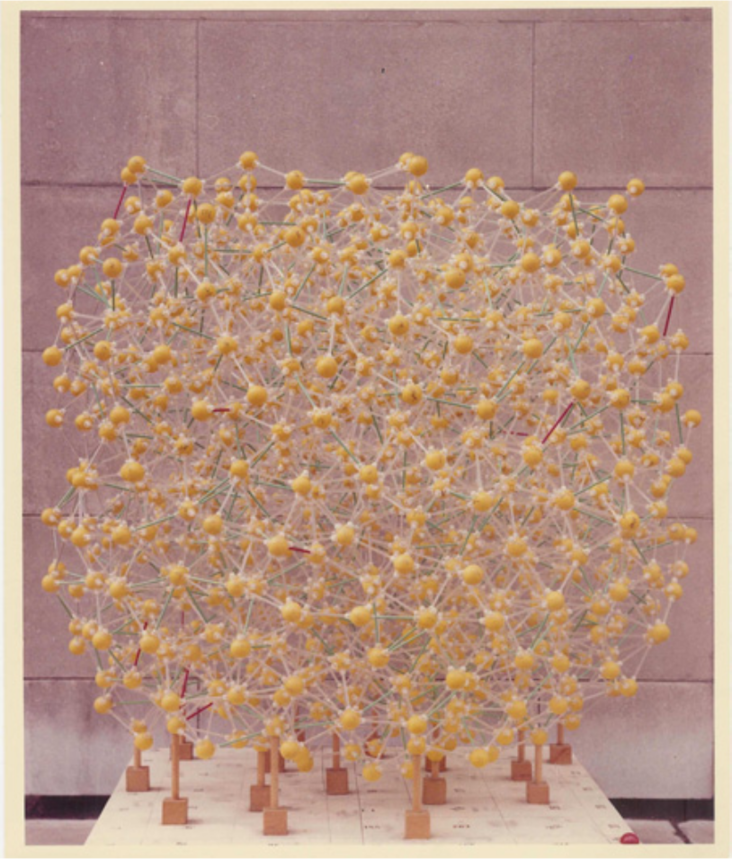
\includegraphics[width=0.38\textwidth]{Figures/WaterModel.png}
  \end{center}
  \caption{Example of an expanded model of a simple liquid (J L Finney, Ph.D thesis)}
\end{wrapfigure}

Simulations have a rich history within physics and engineering, starting even before the
invention of the computer. An example of one of these mechanical simulations is the
 Waterloopkundig Laboratorium or currently the waterloopbos, a scale model of important
Dutch waterways where the influence of waves on harbours and docks was studied. This
simulation played an important part in the design of the famous Delta Works.\\
Another example is the use of mechanical simulations to study the structure of water. In
the early 20th century physicist J.D. Bernal and his fellow researches build various ball
and stick models of water to analyse the possible 3D configurations of water molecules in
a liquid. Their research eventually explained the peculiar physical properties
of water from a atomistic perspective. However useful these mechanical simulations turned
out to be, the biggest drawback of the method was the extreme cost of labour to construct
them as pointed out by Bernal in his 1962 lecture,

\begin{quote}
\dots I took a number of rubber balls and stuck them together with rods of a
selection of different lengths ranging from 2.75 to 4 inch. I tried to do this in the
first place as casually as possible, working in my own office being interrupted every
five minutes or so and not remembering what I had done before the interruption.
However,\dots
\end{quote}

After the first computer simulations where performed in the Los Alamos labs, the
popularity of simulations rapidly increased. The remarkable explanatory power of
simulations combined with the relative easy construction of computer models lead to a
fast adoption of computer simulations in the scientific community. Within the context of
this thesis, computer simulations are used to study the mechanics of
the DNA Polymer. Due to the high number of atoms in a typical system, it is generally
not possible to find an analytical solution to their equations of motion. In this
context, simulations are often used to gain an insight into the complex dynamics of the
system and guide the developments of more simple approximate theories. The simulations
act as a bridge between the microscopic constituents of the systems and the macroscopic
properties we want to understand.


\subsection{Molecular Dynamics Simulations}
Molecular Dynamics Simulations (MD) is a computer simulation technique, used to analyse
the dynamics of a classical many-body system. In a system with $N$ particles, the
trajectories of are generated by numerically integrating the equations of motion.

\[
    m_i \boldsymbol{\ddot{r_i}} = \boldsymbol{f_i}, \quad \boldsymbol{f_i} = -
    \frac{\partial}{\partial \boldsymbol{r_i}} \mathcal{U}
\]
- thermostats

- Integrations schemes

- Rare event sampling

\begin{algorithm}
    \SetKwFunction{isOddNumber}{isOddNumber}
    \SetKwInOut{KwIn}{Input}
    \SetKwInOut{KwOut}{Output}

    \KwIn{Configuration of the system at $t=0$}
    \KwOut{Configuration of the system at $t=t_{f}$}

    $newList = [\ ]$

    \tcc{For odd elements in the list, we add 1, and for even elements, we add 2.
    After the loop, all elements are even.}
    \For{$i \leftarrow 0$ \KwTo $n-1$}{
        \eIf{$\isOddNumber(a_i)$}{

            $newList.append(a_i + 1)$ \tcp*[f]{Some thought-provoking comment.}
         }{
            \tcp{Another comment}
            $newList.append(a_i + 2)$
         }
    }

    \KwRet{$newList$}
    \caption{The Velocity Verlet algorithm}
\end{algorithm}

% \begin{center}
% 	\begin{tikzpicture}[
% 	squarednode/.style={rectangle, draw=blue!60, fill=blue!5, very thick, minimum width=50mm,
% 	minimum height=5mm},]
% 	%Nodes
% 	\node[squarednode]      (step1)                        {1};
% 	\node[squarednode]      (step2)       [below= 3mm of step1] {2};
% 	\node[squarednode]      (step3)       [below= 3mm of step2] {3};
% 	\node[squarednode]      (step4)       [below= 3mm of step3] {4};
% 	\node[squarednode]      (step5)       [below= 3mm of step4] {5};
% 	\node[squarednode]      (step6)       [below= 3mm of step5] {6};
% 	\node[squarednode]      (step7)       [below= 3mm of step6] {7};
% 	\node[squarednode]      (step8)       [below= 3mm of step7] {8};
%
% 	%Lines
%     \draw[very thick, ->] (step1.south) -- (step2.north);
% 	\draw[very thick, ->] (step2.south) -- (step3.north);
% 	\draw[very thick, ->] (step3.south) -- (step4.north);
% 	\draw[very thick, ->] (step4.south) -- (step5.north);
%     \draw[very thick, ->] (step5.south) -- (step6.north);
% 	\draw[very thick, ->] (step6.south) -- (step7.north);
% 	\draw[very thick, ->] (step7.south) -- (step8.north);
% 	\draw[very thick, ->] (step8.west)  -- +(-0.4,0) |-(step2.west);
% 	\end{tikzpicture}
% \end{center}

- understanding many body - newtons algorithm
- insight in the dynamics -> simulate trajectories
- recent developments in techniques to simulate trajectories of rare event
-increased computational power
\subsection{Coarse Grained modelling}
